\section{Semantic Deception Annotation}
\label{sec:annotation}

While the linguistic features analyzed in Section~\ref{sec:methodology} capture statistical proxies for deception, they do not classify the \emph{type} of deception employed. To address this, we conducted an LLM-based annotation study on a stratified sample of werewolf messages, leveraging the unique availability of private reasoning as ground truth for intent.

\subsection{Annotation Taxonomy}

We define four categories of deceptive communication:

\begin{enumerate}
\item \textbf{Direct Lie (LIE)}: The message contains an explicitly false statement, such as falsely claiming to be the Seer or fabricating inspection results.
\item \textbf{Misdirection (MISDIRECT)}: The message deflects suspicion toward an innocent player or away from the speaker's werewolf partner without making explicitly false claims.
\item \textbf{Omission (OMIT)}: The message deliberately withholds relevant information that would reveal the speaker's role.
\item \textbf{Truth-as-Strategy (TRUTH)}: The message is factually true but deployed strategically to manipulate other players, such as making accurate observations to build false credibility.
\end{enumerate}

\subsection{Annotation Protocol}

We sampled 2{,}000 werewolf chat messages per model (16{,}000 total), stratified by game day to ensure temporal coverage. Each message was independently annotated by two LLM judges: DeepSeek-V3.1 and Gemini~2.5 Flash-Lite. Annotators received both the public message and the private reasoning, enabling classification based on the model's actual stated intent rather than inference from text alone.

Inter-annotator agreement reached 78.2\% raw agreement and Cohen's $\kappa = 0.584$ (moderate agreement), comparable to human annotation studies on subjective pragmatic tasks~\citep{artstein2008inter}. Agreement was strongest for LIE (F1=0.810) and MISDIRECT (F1=0.832), and weakest for OMIT (F1=0.319), reflecting genuine ambiguity in distinguishing strategic silence from other strategies. When excluding the rare and ambiguous OMIT category ($<$1\% of labels), the three-class $\kappa$ (LIE/MISDIRECT/TRUTH) rises to 0.641, indicating substantial agreement on the primary deception strategies. Disagreements were resolved by selecting the annotation with higher self-reported confidence, yielding 15{,}090 resolved labels.

\subsection{Results}

\paragraph{Deception type distribution.}
The dominant deception strategy across all models was \textbf{misdirection}, accounting for 67.5\% of all werewolf messages (Figure~\ref{fig:deception_types}). Truth-as-strategy comprised 24.5\%, while direct lies represented only 7.5\% of messages. Omission was rare ($<$1\%).

This distribution reveals that AI werewolves overwhelmingly prefer indirect deception---steering conversations and casting suspicion on innocents---over outright fabrication. This finding aligns with the ``best liars change least'' result from Section~\ref{sec:results}: models that succeed at deception do so by blending truthful observations with subtle redirection, not by constructing elaborate false narratives.

\paragraph{Model-level variation.}
Substantial differences emerge across models (Table~\ref{tab:deception_types}). Gemini~3 Pro---the most successful deceiver at 44.6\% WW win rate---employs the most \emph{balanced} strategy: the highest truth-as-strategy rate (44.0\%) combined with substantial direct lies (12.1\%) and the lowest misdirection dependence (43.6\%). This suggests that effective deception requires a diverse repertoire rather than over-reliance on any single strategy.

At the other extreme, GPT-5.2 is almost entirely misdirection (89.1\%), with negligible lies (1.2\%) and very little truth-as-strategy (9.5\%). GPT-5~mini similarly over-relies on misdirection (83.9\%) while rarely lying (0.6\%)---and achieves the worst win rate (13.6\%). The GPT family's aversion to outright lying may reflect stronger RLHF alignment against producing false statements, but this constraint appears to \emph{hurt} deceptive performance by making their strategy predictable.

Grok~4 presents a striking profile: high lying (12.3\%) \emph{and} high misdirection (80.5\%), but almost no truth-as-strategy (7.0\%). This aggressive but one-dimensional approach yields only moderate success (22.1\%). The Claude models occupy a middle ground, with Sonnet~4.5 showing more willingness to lie (8.7\%) than Opus~4.5 (4.7\%).

\begin{table}[t]
\caption{Deception strategy distribution by model (\%). Models sorted by WW win rate. Gemini~3 Pro (highest win rate) uses the most balanced mix; GPT-5.2 and GPT-5~mini over-rely on misdirection.}
\label{tab:deception_types}
\centering
\small
\begin{tabular}{lcccc|c}
\toprule
\textbf{Model} & \textbf{LIE} & \textbf{MISDIR.} & \textbf{OMIT} & \textbf{TRUTH} & \textbf{WW Win Rate} \\
\midrule
Gemini 3 Pro     & 12.1 & 43.6 & 0.3 & 44.0 & 44.6 \\
GPT-5.2          &  1.2 & 89.1 & 0.3 &  9.5 & 37.8 \\
Gemini 3 Flash   & 12.6 & 50.5 & 0.3 & 36.6 & 37.7 \\
Claude Opus 4.5  &  4.7 & 64.9 & 1.0 & 29.4 & 36.0 \\
Claude Sonnet 4.5 & 8.7 & 54.0 & 1.2 & 36.1 & 35.8 \\
Grok 4.1 Fast    &  7.5 & 73.6 & 0.7 & 18.2 & 24.4 \\
Grok 4           & 12.3 & 80.5 & 0.1 &  7.0 & 22.1 \\
GPT-5 mini       &  0.6 & 83.9 & 0.1 & 15.4 & 13.6 \\
\midrule
\textbf{Overall} & \textbf{7.5} & \textbf{67.5} & \textbf{0.5} & \textbf{24.5} & --- \\
\bottomrule
\end{tabular}
\end{table}

\begin{figure}[t]
\centering
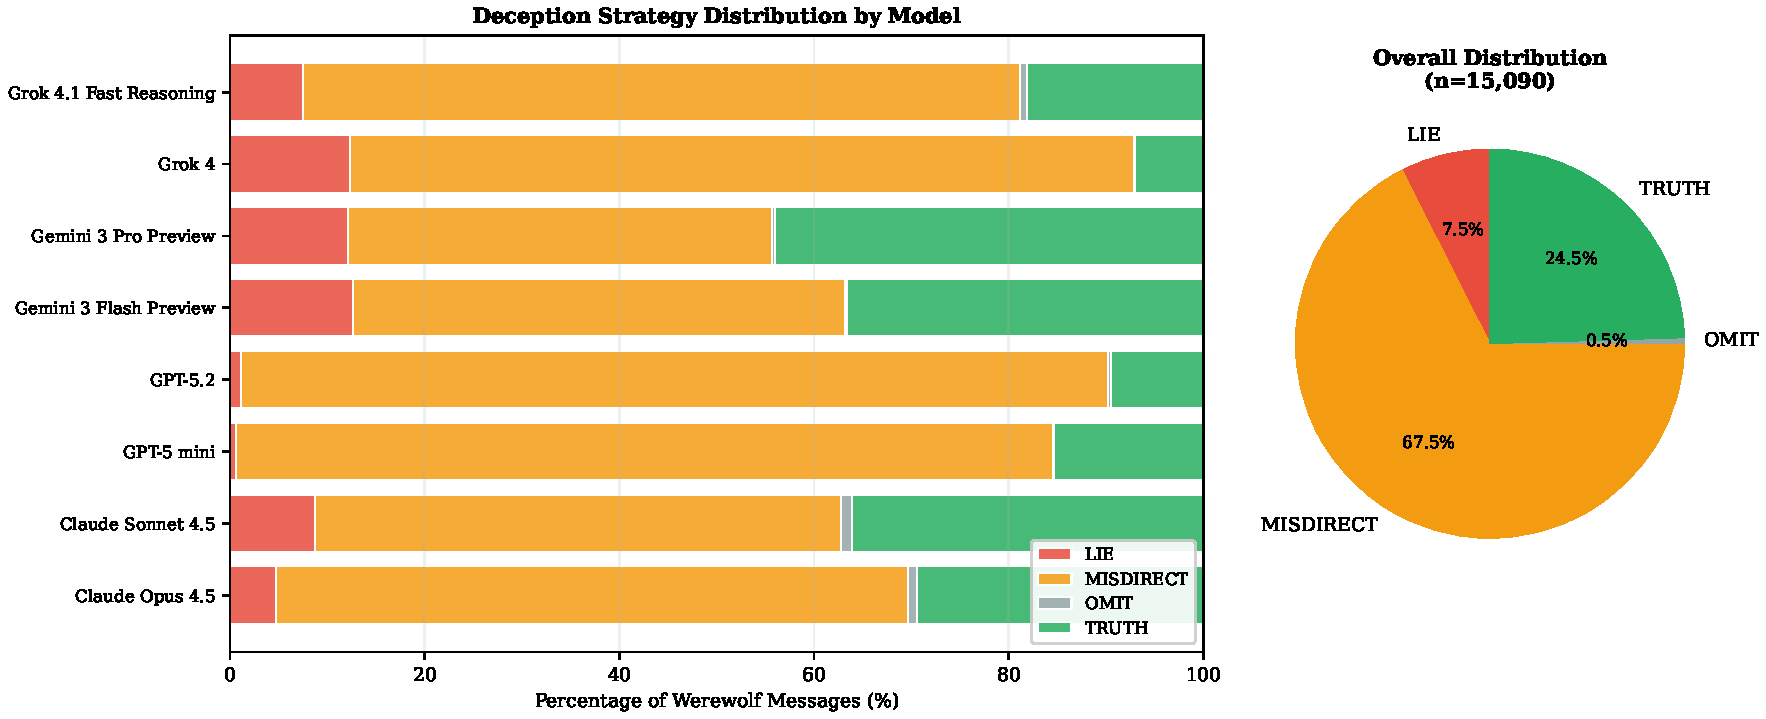
\includegraphics[width=\textwidth]{figures/fig6_deception_types.pdf}
\caption{Deception strategy distribution by model. GPT-family models overwhelmingly favor misdirection, while Gemini~3 Pro employs the most balanced repertoire---correlating with the highest werewolf win rate.}
\label{fig:deception_types}
\end{figure}

\paragraph{Temporal dynamics.}
As games progress, werewolves shift toward more aggressive deception (Figure~\ref{fig:deception_temporal}). Direct lies increase from 4.6\% on Day~1 to 10.7\% by Day~3, while truth-as-strategy decreases substantially (31.0\% $\to$ 19.4\%). Misdirection increases from 63.8\% to 69.6\%. This pattern suggests that surviving werewolves face increasing pressure to fabricate as the player pool shrinks and scrutiny intensifies---a dynamic that mirrors human behavior in social deduction games.

\begin{figure}[t]
\centering
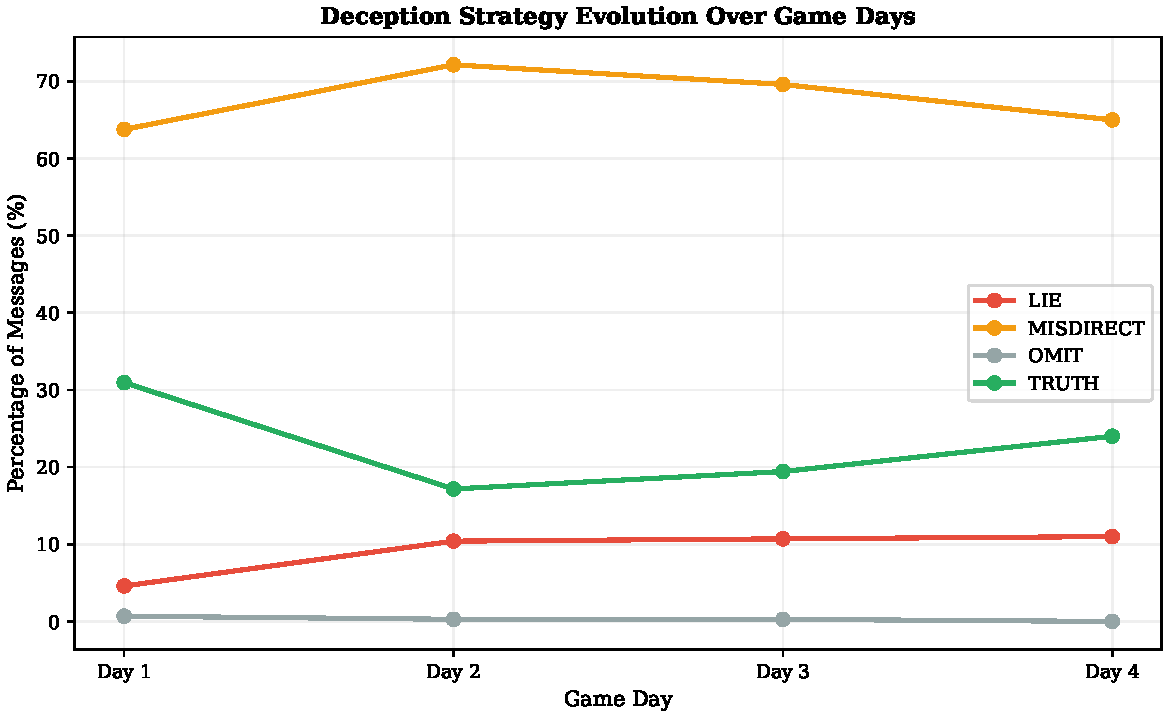
\includegraphics[width=0.9\textwidth]{figures/fig7_deception_temporal.pdf}
\caption{Evolution of deception strategies over game days. As games progress and scrutiny intensifies, werewolves shift from truth-as-strategy toward direct lies and misdirection.}
\label{fig:deception_temporal}
\end{figure}
